\cleardoublepage
\mbox{}

\lstset{
language=Python,
basicstyle=\small\sffamily,
numbers=left,
numberstyle=\tiny,
frame=tb,
columns=fullflexible,
showstringspaces=false
}

\chapter{Implementación}
\label{ch:chapter4}
La implementación de la aplicación y la puesta en producción de esta se materializa en un entorno cloud, en concreto Google Cloud Platform
Los servicios que proporciona Google Cloud\footnote{https://cloud.google.com/} son de especial utilidad para el problema debido a que muchos de ellos son mantenidos y actualizados por la propia
plataforma, por lo que no hay que dedicar especial esfuerzo a configurar estos servicios, más que la primera vez que vayamos a utilizarlos o cuando se quiera
modificar cualquier parámetro de configuración.
Otra de las grandes ventajas de usar este tipo de implementación cloud es que podemos escalar nuestras
aplicaciones casi de manera infinita según la demanda de nuestro aplicación.
A diferencia del resto de aplicaciones mencionadas hasta el momento, los servicios de google son de pago, en muchos de ellos existe una modalidad gratuita pero los recursos de estas
están limitadas en su capacidad de trabajo o en el tiempo que se pueden usar .


\section{Descripción del entorno y sus diferentes componentes}\label{sec:descripción-del-entorno-y-sus-diferentes-componentes}
Las diferentes piezas que constituyen nuestra arquitectura cloud son las siguientes.

\subsection{Google Storage}\label{subsec:storage}
Es el sistema de almacenamiento de Google.
Su objetivo dentro de la aplicación es poder ser utilizada como sistema de copia de seguridad de todas las imágenes que se vayan procesando, así como también de disparador para procesar dicha
imagen en el pipeline del proceso principal y poder clasificarla, ya que el servicio incorpora eventos automáticos cada vez que un archivo se ha descargado, subido o modificado.
Esta solución es la principal entrada de datos de la aplicación, por lo que nadie sin una clave de autenticación específica del proyecto puede subir archivos.
Las características principales que se han encontrado en el uso de esta aplicación para el trabajo son :
\begin{itemize}
    \item Escalabilidad practicamente infinita en el volumen de almacenamiento de los archivos.
    \item Posibilidad de configurar distintas ubicaciones o múltiples para almacenar los datos, de modo que se pueden tener réplicas del historial en distintas partes del mundo de manera simultánea.
    La replicación de los nodos a través de las distintas ubicaciones y su consistencia es una ventaja totalmente gestionada por Google.
    \item Opción de carga en paralelo, la cual ha sido utilizada para los benchmark de la aplicación.
    \item Encriptación de los datos y restricción de los accesos a los archivos de forma individual o colectiva.
    \item Interoperabilidad con el resto de servicios cloud.
\end{itemize}

\subsection{Google BigQuery}\label{subsec:bigquery}
Es una base de datos columnar y distribuida mantenida por Google, de modo que no hay que configurar su funcionamiento interno.
En la aplicación de este trabajo BigQuery funciona como herramienta de análisis y exploración de los resultados obtenidos en las distintas pruebas de carga.
Todos los conjuntos de datos de esta base de datos han sido configurados en Europa para disminuir la latencia lo máximo posible.
Las razones principales de su uso son :
\begin{itemize}
    \item Capacidad de análisis del orden de Petabytes en cuestión de segundos debido a los múltiples nodos que ejecutan las cargas de trabajo de manera distribuida.
    \item Posibilidad de almacenar los distintos conjuntos de datos en ubicaciones distintas, reduciendo así la latencia dependiendo del sitio donde se ejecuten los trabajos.
    \item Soporte para la ingesta de datos en tiempo real.
    \item Acceso a distintas API en varios lenguajes de programación.
    \item Uso de SQL estándar como lenguaje de consulta.
\end{itemize}

\subsection{Google Pub/Sub}\label{subsec:pubsub}
Es un sistema de colas de mensajería diseñada para eventos,
stá basado en el patrón de diseño productor/consumidor.
En esta arquitectura cloud servirá de hilo conductor para las distintas partes de la aplicación cada vez que se produzca un evento como el de una nueva carga de imagen o la petición al servidor para realizar la clasificación.
Sus caracteríscas se pueden enumerar en :

\begin{itemize}
    \item Se pueden configurar distintas colas de mensajes, separando así de manera lógica los eventos de la aplicación.
    \item Este tipo de eventos está pensado para ser consumido en tiempo real, con la mínima latencia posible.
    \item Soporte para la ingesta de datos en tiempo real.
\end{itemize}

\subsection{Google Compute Engine}\label{subsec:computeengine}
Es el servicio principal de Google para proporcionar máquinas virtuales totalmente configurables, tanto en su capacidad de cálculo seleccionando el tipo de procesador, gpu y memoria ram que se necesite, como en el entorno
en el que se va a ejecutar la aplicación, ya sea docker o las distintas distribuciones de sistemas operativos.
Este servidor usará como aplicación principal una imagen de docker almacenada en el registro de contenedores.
Este instrumento será el principal ejecutor de la aplicación, procesando y clasificando las nuevas imágenes que se carguen en el sistema de almacenamiento y volcando el resultado a la base de datos.

\subsection{Google Cloud Function}\label{subsec:cloudfunction}
Este sistema nos permite ejecutar una pequeña porción de código en el mínimo tiempo posible en una máquina virtual activada por eventos.
Estas máquinas escalan bajo demanda y no tienen que encenderse o apagarse cada vez que reciben una petición, por lo que siempre y están disponibles y no hay apenas latencia.
En esta aplicación servirán de puente entre el volcado de una imagen al sistema de almacenamiento y el procesamiento de la petición al servidor con la información y metadatos correspondientes para realizar
la clasificación.

\subsection{Container Registry}\label{subsec:container-registry}
Dado que todo el desarrollo de la aplicación y el versionado de esta ha sido efectuado mediante docker se ha usado
un repositorio de imágenes para el almacenamiento y tagueado de estas.
En este repositorio se almacenan las distintas imágenes de docker tanto para openvino como para tensorflow, ya que se han
separado lógicamente para optimizar el tamaño de la imágen origen que tiene cada una de las aplicaciones.


En la siguiente figura\ref{fig:Arquitectura Google Cloud} podemos observar una imagen completa de la arquitectura mencionada anteriormente y el flujo de trabajo
que seguiría una imagen desde que es volcada en el sistema de almacenamiento hasta que su clasificación es almacenada en la base de datos
para su análisis.

\begin{figure}
    \centering
    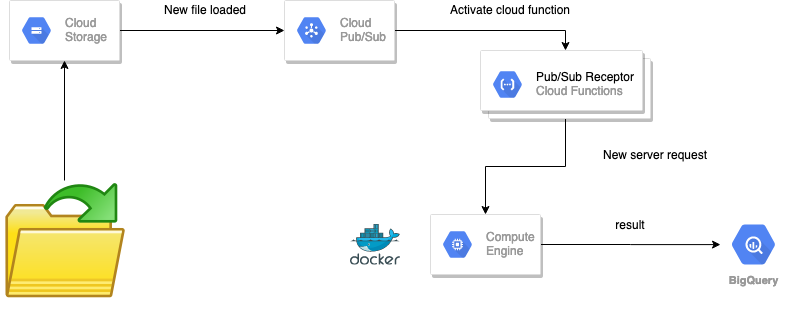
\includegraphics[width=0.8\textwidth]{images/chapter4/cloud_architecture.png}
    \caption{Arquitectura Google Cloud}
    \label{fig:Arquitectura Google Cloud}
\end{figure}

\section{Codificación de los servidores web}\label{sec:codificación-de-los-servidores-web}
Con el objetivo de poder procesar todas las peticiones y recoger todos los metadatos necesarios para el su posterior análisis se necesita codificar un servidor web que realice todo este trabajo.
Para ello se ha elegido, como anteriormente, el lenguaje de programación Python debido a la creciente comunidad actual en el mundo de la informática y el desarrollo software, lo que hace que el nivel
de información sobre desarrollo con este lenguaje sea significativamente más alto que otros lenguajes.
Se ha empleado un paradigma de programación orientado objetidos debido a la organización que proporciona con aplicaciones de un tamaño considerable y la dotación de intedidad que facilita a los distintos
componentes.
Debido a la multitud de framework web actuales se han elegido varios para su puesta a prueba en la aplicación.
Para el procesamiento generalizado de imágenes y el sistema de recogia de metados se han codificado dos clases princpales.
La primera\ref{lst:api}, encargada de la inicialización de los servicios de GoogleStorage y GoogleBigQuery, para los cuales se han codificado métodos para descarga y carga de información respectivamente.
Se presenta un método principal para procesar las peticiones al servidor, que modela toda la información que va a ser incluida en la base datos.
Esta información consta de los siguientes campos :

\begin{itemize}
    \item Nombre de la imagen
    \item Tipo de archivo, que especifica el formato del fichero.
    \item Fecha exacta de creación del archivo en el sistema de almacenamiento.
    \item Clasificación de la imagen, para saber si el terreno de esta está dañado o no.
    \item Tiempo de inferencia en la red.
    En este caso dependerá de si estamos usndo openvino o tensorflow para realizar esta tarea.
    \item Tiempo total de ejecucón desde que se que llega una petición al servidor hasta que se procesa.
    \item Número de núcleos físicos del procesador.
    \item Número de núcleos virtuales del procesador.
    \item Sistema operativo
    \item Versión del sistema operativo.
    \item Memoria ram del sistema.
    \item Sistema de inferencia, en este caso puede ser openvino o tensorflow.
    \item Framework web utilizado, flask o fastapi en esta apliación.
    \item Campo booleano para determinar si se está usando docker para encapsular la aplicación.
    Para realizar las pruebas siempre se ha usado docker.
    \item Campo booleano para saber si la aplicación se está ejecutando en un entorno local o en cloud.
    En este caso siempre se ejecuta la aplicación en un entorno cloud.
\end{itemize}


\begin{lstlisting}[caption=Api, label=lst:api, float=h]
    class Api:
    def __init__(self, net, sys: SystemTrack):
        self.__storage = GoogleStorage()
        self.__big_query = GoogleBigQuery()
        self.__net = net
        self.sys_track = sys

    def cloud_storage_request(self, item: dict):
        start = time.time()
        image_name = item['name']
        size = item['size']
        file_type = item['contentType']
        time_created = item['timeCreated']
        image_path = f'{data_dir}{image_name}'
        self.__storage.download_blob(bucket, image_name, image_path)
        prediction, inference_time = self.__net.process_image(image_path)
        total_time = time.time() - start
        row = [
            (
                image_name, size, file_type,
                time_created, prediction, inference_time,
                total_time, self.sys_track.physical_cores,
                self.sys_track.total_cores, self.sys_track.system, self.sys_track.processor,
                self.sys_track.system_memory,
                self.sys_track.system_memory_available,
                self.sys_track.so_version, self.sys_track.so_release, self.sys_track.inference_engine,
                self.sys_track.web_engine, self.sys_track.processor_unit,
                self.sys_track.docker, self.sys_track.cloud
            )
        ]
        self.__big_query.insert_row(row)
        os.remove(image_path)
\end{lstlisting}
La segunda refclase clase es la encargada de generar y recabar toda esta información para que la clase Api pueda procesarla.
Se ha hecho uso de las librerías de psutil \footnote{ https://pypi.org/project/psutil/} y platform {https://docs.python.org/3/library/platform.html} para conseguir la información necesaria del sistema.
Contamos de manera adicional con un método de conversión de unidades para normalizar los datos a un estándar preestablecido.
Este objeto de tipo SystemTrack es el que será enviado por argumento a la clase Api, la cual procesará todos estos datos.
\begin{lstlisting}[caption=Api, label=lst:system, float=h]
class SystemTrack:
    def __init__(self, docker: bool, inference_engine: str, web_engine: str, cloud: bool, processor_unit: str):
        self.sys_information = platform.uname()
        self.sys_memory = psutil.virtual_memory()
        self.physical_cores = psutil.cpu_count(logical=False)
        self.total_cores = psutil.cpu_count(logical=True)
        self.system = self.sys_information.system
        self.processor = self.sys_information.processor
        self.system_memory = self.__get_size(self.sys_memory.total)
        self.system_memory_available = self.__get_size(self.sys_memory.available)
        self.so_version = self.sys_information.version
        self.so_release = self.sys_information.release

        self.docker = docker
        self.inference_engine = inference_engine
        self.web_engine = web_engine
        self.cloud = cloud
        self.processor_unit = processor_unit

    @staticmethod
    def __get_size(num_bytes, suffix="B"):
        factor = 1024
        for unit in ['', 'K', 'M', 'G', 'T', 'P']:
            if num_bytes < factor:
                return f'{num_bytes:.2f}{unit}{suffix}'
            num_bytes /= factor
\end{lstlisting}
\subsection{Framework FastApi}\label{subsec:framework-fastapi}
FastApi \footnote{https://fastapi.tiangolo.com/} es un framework web de alto rendimiento preparado para su puesta en producción.
Las características principales de este framework son las siguientes :

\begin{itemize}
    \item Desarrollo rápido debido a la arquitectura de componentes del framework.
    \item Documentación detallada para componente.
    \item Incorpora un sistema de tipado de objetos para su fácil identificación.
    \item Estándar OpenApi\footnote{https://github.com/OAI/OpenAPI-Specification} para la especificación del formato de las peticiones entrantes y las respuestas del servidor.
\end{itemize}

Para soportar este framework se usará Uvicorn \footnote{https://www.uvicorn.org/} como servidor ASGI \footnote{https://asgi.readthedocs.io/en/latest/} (Asynchronous Server Gateway Interface), lo que significa que el servidor puede procesar tanto peticiones asíncronas como síncronas.
Ademas, nos proporcionará las herramientas necesarias para paralelizar la carga de las peticiones
entre los distintos nodos e hilos de la aplicación, adicionalmente se dispondrán de opciones de configuración de certificados SSL, logs y puerto por el que funciona la apliación dentro del host.
Este servidor soporta actualmente el protcolo de transmisión de datos HTTP/1.1 y está preparado para recibir peticiones asíncronas.
Este software es de código abierto y podemos encontrar su código fuente en su repositorio oficial

\subsection{Framework Flask}\label{subsec:framework-flask}
Flask \footnote{https://flask.palletsprojects.com/en/1.1.x/} es el framework ligero por excelencia de Python , está desarrollado de manera sencilla y ligera, diferenciándose así de otros frameworks pesados como Djando, que incluyen
muchas dependencias y acaban ocupando mucho espacio en disco y en memoria.

A diferencia de fastapi Flask se centra en la simplicidad de sus elementos y dota a sus usuarios se una serie de interfaces y decoradores simples para su codificación.
Como servidor web se usará Gunicorn \footnote{https://gunicorn.org/} que sigue el estándar WSGI \footnote{https://en.wikipedia.org/wiki/Web\_Server\_Gateway\_Interface} (Web Server Gateway Interface), que es una convención simple para gestionar llamadas síncronas al servidor.
Con este servidor podremos seleccionar la paralelización y distribución de carga del procesador.


\section{Encapsulación de entorno con Docker}\label{sec:encapsulación-de-entorno-con-docker}
En la siguiente figura~\ref{fig:Arquitectura de la máquina virtual de la aplicación} podemos observa la arquitectura para ambos frameworks que se desplegarán en las máquinas virtuales de Google.

\begin{figure}
    \centering
    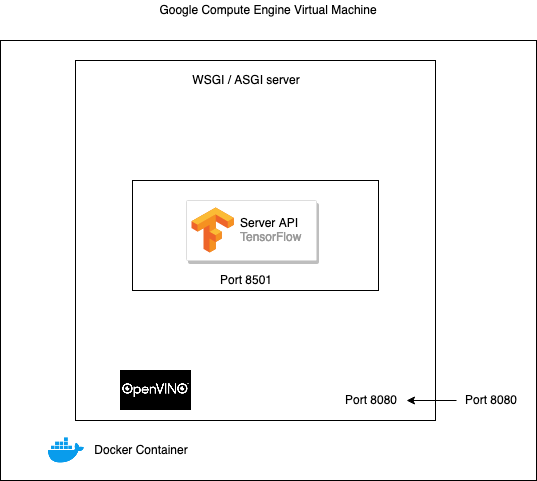
\includegraphics[width=0.8\textwidth]{images/chapter4/host_architecture.png}
    \caption{Arquitectura de la máquina virtual de la aplicación}
    \label{fig:Arquitectura de la máquina virtual de la aplicación}
\end{figure}

Buscando la máxima portabilidad entre entornos y no cerrar la posibilidad de traslado de estas a otra plataforma se han ecapsulado todas las aplicaciones
usando la tecnología de contenedores docker \footnote{https://www.docker.com/}.
Este contenedor de docker se conectará con el host mediante el puerto 8080, pertimitiendo así el tráfico de información.
Dentro del mismo se levantarán los correspondientes servidores WSGI o ASGI dependiendo de si estamos usando flask o fastapi respectivamente.
Es necesario clarificar que nunca habrá dos servidores activos al mismo tiempo, por lo que se dispondrán de distintas versiones de las aplicaciones en el registro de contenedores
preparadas para usar cada servidor de manera independiente.
Dentro de estos contenedores y dependiendo de la aplicación a usar se puede encontrar directamente la aplicación de inferencia de Openvino, la cual funcionará de manera directa o por el contrario,
si usamos tensorflow tendremos otro servidor rest api que procesará las peticiones dentro del contenedor por el puerto 8501.
De igual modo que los servidores nunca existirá la posibilidad de tener instalados en el mismo servidor openvino y tensorflow a la vez, independizando su uso según los requisitos y necesidades del usuario.
Se han versionado las siguientes imágenes para la aplicación :
\begin{itemize}
    \item Imagen para la aplicación de entrenamiento del modelo de deep learning, que ha sido utilizada para realizar pruebas de concepto en un entorno de desarrollo local antes de usar su funcionalidad
    interna en Google Colab.
    Se ha encontrado útil su uso debido a que el proceso de desarrollo se ha llevado acabo en distintos entornos y sistemas operativos como MacOS, Windows o Linux dependiendo de las necesidades del programador.
    \item Imagen para la red de inferencia de openvino, que contiene las librerías necesarias para su ejecución y puesta en producción.
    \item Imagen para la red de inferencia de tensorflow, configurando el servidor interno que proporciona las inferencias al contenedor, y este, a la base de datos.
\end{itemize}

Para la construcción de estas imágenes se han codificado de manera explícita cada una de ellas y constan en el repositorio de este trabajo \footnote{https://github.com/A-Ortiz-L/multispectral-imaging-cnn-final-degree-work/tree/master/docker}
En la configuración de estas se especifican los siguientes puntos :
\begin{itemize}
    \item Sistema operativo base o imagen de la que hereda el contenedor.
    \item Puertos necesarios para ejecutar la aplicación, que son expuestos al exterior.
    \item Paquetes y actualizaciones del sistema operativo necesarios para funcionar.
    \item Librerías de python.
    \item Variables de entorno del sistema operativo.
    \item Código y ficheros que se van a incluir en la imagen.
\end{itemize}

Como herramienta adicional y enlazada al uso de docker se ha utilizado docker compose \footnote{https://docs.docker.com/compose/} para las pruebas de funcionamiento y testeo de todas estas imágenes.
Con esta aplicación podemos describir exactamente cómo se va a ejecutar cada una de las imágenes de docker y los comandos que queremos que se ejecuten de manera automática al iniciarse el contenedor.

